\label{chap4}

This chapter details the controller design of the model based controller. The performance of the controller is tested with the aid of a simulation model. The model as derived in Chapter \ref{chap2} will be used with the parameters found in Chapter \ref{chap3}. In order for the model to be complete pump dynamics should be added. These pumps have a major influence on the dynamics of the system. Once these are determined the Jacobian controller can be implemented on the dynamic model. 


\section{Jacobian control}


The controller designed in this study includes jacobian information. Jacobian control is a widely used type of model-based controller for positioning classic robots. As mentioned in Chapter \ref{chapter1}, jacobian controllers only use model information on velocity and position level. Thus, system dynamics are not used in this control law.


The Jacobian controller proposed is an adapted version of the one presented in \cite{MOOSAVIAN20071226}. This work shows that a computed torque controller can be approximated by a more straightforward control law involving the Jacobian transpose. This approximation holds if high enough control gains are used. The mentioned research only uses a proportional and derivative action to reduce the error. In order to remove the steady-state error, an integrator gain is added this controller. This Jacobian transposed control law is given by,


\begin{equation}
    \tau_{set} = \begin{bmatrix}J(\sigma,t)\end{bmatrix}^\top \Big(K_p e + K_i \int_0^t e \hspace{2pt} ds \Big), 
    \label{eq:tau}
\end{equation}

where $\tau_{set} \in \mathbb{R}^2$ is the control input vector with control input moment and force. The Jacobian is determined with equation \ref{eq2:J}. Furthermore, $K_p$ and $K_i \in \mathbb{R}^{2\times 2}$ are diagonal gain matrices. Here $K_p$ penalizes proportional to the error, $K_i$ contributes to the sum of the error over time. The error $e \in \mathbb{R}^2$ is defined as the difference between reference position and the actual position in the (x,y)-plane. Therefore not the entire Jacobian of dimension $6 \times 2$, but only the entries mapping modal coordinate velocity to linear velocity in x-y plane. These are the fourth and sixth row of the Jacobian. As mentioned this Jacobian is space-time variant. Therefore, in the control law this Jacobian is calculated real-time based on the actual kinematic configuration of the actuator. 

The actual system does not allow to induce forces and moments directly. Therefore this control input should be mapped to pressure. Here the mapping as found with finite element analysis in Chapter \ref{chap3} is used to map pressure to force. Based on the desired control input, a reference pressure can be formulated as,

\begin{equation}
    p_{ref} = H^{-1}\tau,
\end{equation}


where $p_{ref} \in \mathbb{R}^2$ is the reference pressure for each bellow. In order for this reference pressure to be reached a second controller is necessary. This low-level controller is used to set the input voltage that is supplied to the pumps.  The volt input is regulated via pulse width modulation (pwm). Since the Raspberry PI is equipped with a 12bit ADC (analog-digital converter), it is possible calculate the pwm input as, $\textit{pwm} = \frac{2^{12} V}{V_{max}} $, where $V_{max}$ is equal to 12 volt. This control law is given by,


\begin{equation}
    pwm_{set} = K_{pp}e_p \hspace{10pt} \text{with} \hspace{10pt} e_p = p_{ref} - p,
\end{equation}



where $pwm_{set}$ is the input voltage and $K_{pp} \in \mathbb{R}^{2\times 2}$ a diagonal gain matrix. Furthermore, $e_p$ is the pressure error, which is the difference between reference pressure and actual pressure. Observe that only a proportional action is used. The integral action of the jacobian controller will already ensure no steady-state error. 




where state vector $x$ is extended to $x = [\kappa \hspace{3pt} \epsilon \hspace{3pt} \dot{\kappa} \hspace{3pt} \dot{\epsilon} \hspace{3pt} p_1 \hspace{3pt} p_2]$. Here matrix $A \in \mathbb{R}^{6\times 6}$ containing the dynamics is extended. Additionally input matrix $B \in \mathbb{R}^{6\times 4}$ is extended to allow volt input. In this simulation model, the volt input is limited to be between 0 and 12 volt. This constrains the system such that negative pressures can not be used to control the system. 

\hl{Here I would like to add simulations of the jacobian controller. I also would like to include model simulations using stiffness compensation. Some simulations are carried out, but are still incomplete and are therefore not included in this draft.}

%Above state space model and presented Jacobian controller is implemented in \MATLAB. The used settings gains are $K_p = \text{diag}([400,400])$  and $K_i = \text{diag}([150,150])$. Figure  shows a simulation for a set point $q_{set} = [0 0.3]^\top$, which is equivalent to a position of [0,0.084]$m$ in the xy-plane.




%It is clear that since only a elongation is desired the pressure in both bellows should become equal. Therefore control input $V_1 = V_2$, and is saturated to the maximum 12V. Once the setpoint is nearly reached the control input slowly drops to ... V. It can be seen that the pump dynamics are the major limiting factor in the achievable performance of the set-up. The dynamic model simulations shown in Appendix \ref{app4} showed that for a free oscillation the settling time is in the order of 0.1 seconds. For this setpoint the settling time is around ... seconds. Clearly the actuator damping does not play a large role setpoint regulation. . As one can see the controller  


%Using the same tuning parameters a curvature set-point as $q_{set} = [10,0.3]$ can be simulated. 


%\begin{figure}
%    \centering
%    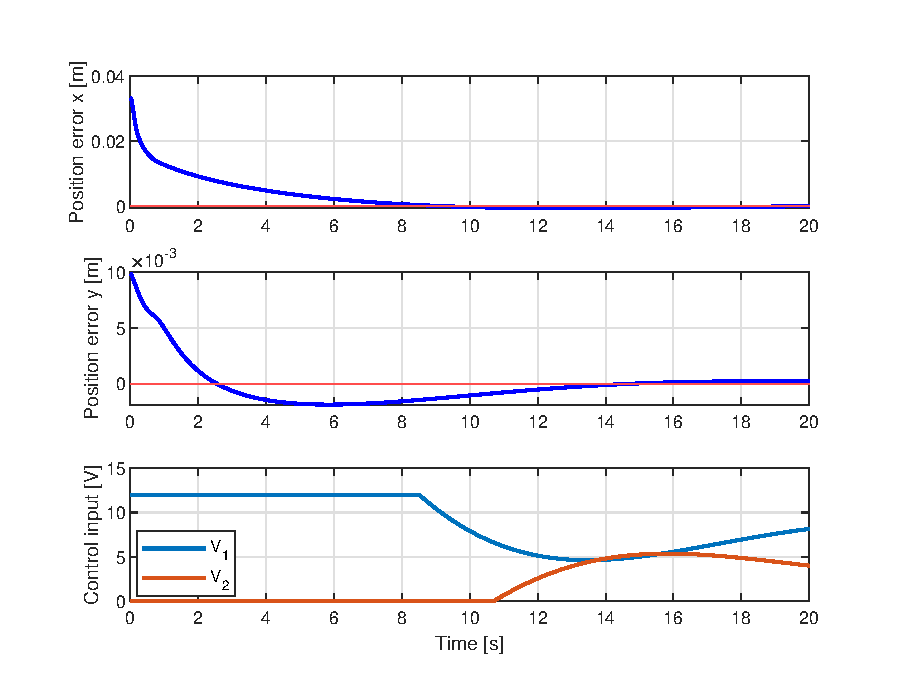
\includegraphics{Figures/Chapter4/k10e03.eps}
 %   \caption{Caption}
%    \label{fig:my_label}
%\end{figure}


























%The proposed Jacobian controller can be improved by adding additional model information. A major improving factor to the performance of the controller is adding stiffness compensation. Since the set-point is known, the necessary stiffness force and moment at that position are known. This compensation can directly be added to the control signal. The resulting controller then is,


%\begin{equation}
  %  \tau_{set} = \begin{bmatrix}J(\sigma,t)\end{bmatrix}^\top \Big(K_p e %+ K_i \int_0^t e \hspace{2pt} ds +  K_d \dot{e}\Big) + %\begin{bmatrix} K_\kappa(\kappa_{set}) & 0 \\ 0 & %K_\epsilon(\epsilon_{set}) \end{bmatrix} q_{set} , 
%    \label{eq:tauK}
%\end{equation}

%where additionally the stiffness is evaluated at modal coordinate setpoint $q_{set}$